In this section we present the experimental setup and explain the different measurements done.
\subsection{Experimental Setup}
The complete setup for the lifetime measurement can be found in figure \ref{fig:setup}. The different inputs and outputs are not marked explicitly but should be clear from the context. L (R) stands for the left (right) detector. The setup is configurated step for step, beginning at the detectors. 

\begin{figure}[h]
  \centering
  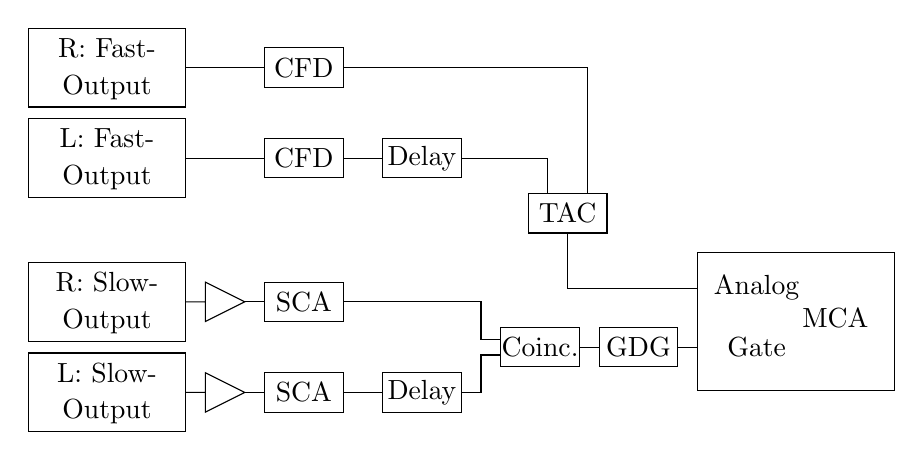
\begin{tikzpicture}
    \draw (-9,-1.25-1.6+3.95) rectangle (-7,-0.25-1.6+3.95);
    \draw (-8,-0.5-1.6+3.95) node {R: Fast-};
    \draw (-8,-1-1.6+3.95) node {Output};
    \draw (-7,-0.75-1.6+3.95)--(-1-5,-0.75-1.6+3.95);
    \draw (-1-5,-2.1+3.95) rectangle (-1-4,-2.6+3.95);
    \draw (-1-4.5,-2.35+3.95) node {CFD};
    \draw (-1-4,-2.35+3.95)--(-1-1.4+0.5,-2.35+3.95)--(-1.9,0);
    \draw (-9,-1.25-1.6+2.8) rectangle (-7,-0.25-1.6+2.8);
    \draw (-8,-0.5-1.6+2.8) node {L: Fast-};
    \draw (-8,-1-1.6+2.8) node {Output};
    \draw (-7,-0.75-1.6+2.8)--(-1-5,-0.75-1.6+2.8);
    \draw (-1-5,-2.1+2.8) rectangle (-1-4,-2.6+2.8);
    \draw (-1-4.5,-2.35+2.8) node {CFD};
    \draw (-1-4,-2.35+2.8)--(-1-3.5,-2.35+2.8);
    \draw (-1-3.5,-2.1+2.8) rectangle (-1-2.5,-2.6+2.8);
    \draw (-1-3,-2.35+2.8) node {Delay};
    \draw (-1-2.5,-2.35+2.8)--(-1-1.4,-2.35+2.8)--(-2.4,0);
    \draw (-2.65,0) rectangle (-1.65,-0.5);
    \draw (-2.15,-0.25) node {TAC};
    \draw (-2.15,-0.5)--(-2.15,-1.2)--(-0.5,-1.2);

    \draw (-9,-1.25-1.6+3.95-2.525-0.45) rectangle (-7,-0.25-1.6+3.95-2.525-0.45);
    \draw (-8,-0.5-1.6+3.95-2.525-0.45) node {R: Slow-};
    \draw (-8,-1-1.6+3.95-2.525-0.45) node {Output};
    \draw (-7,-0.75-1.6+3.95-2.525-0.45)--(-6.75,-0.925-0.45)--(-6.75,-1.175-0.45)--(-6.25,-0.925-0.45)--(-6.75,-0.675-0.45)--(-6.75,-0.925-0.45);
    \draw (-6.25,-0.925-0.45)--(-1-5,-0.75-1.6+3.95-2.525-0.45);
    \draw (-1-5,-2.1+3.95-2.525-0.45) rectangle (-1-4,-2.6+3.95-2.525-0.45);
    \draw (-1-4.5,-2.35+3.95-2.525-0.45) node {SCA};
    \draw (-1-4,-2.35+3.95-2.525-0.45)--(-3.25,-2.35+3.95-2.525-0.45)--(-3.25,-1.4-0.45)--(-3,-1.4-0.45);
    \draw (-9,-1.25-1.6+2.8-2.525-0.45) rectangle (-7,-0.25-1.6+2.8-2.525-0.45);
    \draw (-8,-0.5-1.6+2.8-2.525-0.45) node {L: Slow-};
    \draw (-8,-1-1.6+2.8-2.525-0.45) node {Output};
    \draw (-7,-0.75-1.6+2.8-2.525-0.45)--(-6.75,-0.925-1.15-0.45)--(-6.75,-1.175-1.15-0.45)--(-6.25,-0.925-1.15-0.45)--(-6.75,-0.675-1.15-0.45)--(-6.75,-0.925-1.15-0.45);
    \draw (-6.25,-0.925-1.15-0.45)--(-1-5,-0.75-1.6+2.8-2.525-0.45);
    \draw (-1-5,-2.1+2.8-2.525-0.45) rectangle (-1-4,-2.6+2.8-2.525-0.45);
    \draw (-1-4.5,-2.35+2.8-2.525-0.45) node {SCA};
    \draw (-1-4,-2.35+2.8-2.525-0.45)--(-1-3.5,-2.35+2.8-2.525-0.45);
    \draw (-1-3.5,-2.1+2.8-2.525-0.45) rectangle (-1-2.5,-2.6+2.8-2.525-0.45);
    \draw (-1-3,-2.35+2.8-2.525-0.45) node {Delay};
    \draw (-1-2.5,-2.35+2.8-2.525-0.45)--(-3.25,-2.35+2.8-2.525-0.45)--(-3.25,-1.6-0.45)--(-3,-1.6-0.45);
    \draw (-3,-1.75-0.45) rectangle (-2,-1.25-0.45);
    \draw (-2.5,-1.5-0.45) node {Coinc.};
    \draw (-2,-1.5-0.45)--(-1.75,-1.5-0.45);
    \draw (-1.75,-1.75-0.45) rectangle (-0.75,-1.25-0.45);
    \draw (-1.25,-1.5-0.45) node {GDG};
    \draw (-0.75,-1.95)--(-0.5,-1.95);

    \draw (-0.5,-2.5) rectangle (2,-0.75);
    \draw (1.25,-1.575) node {MCA};
    \draw (0.25,-1.95) node {Gate};
    \draw (0.25,-1.2) node {Analog};
  \end{tikzpicture}
  \caption{Setup for the lifetime measurement.}
  \label{fig:setup}
\end{figure}

\subsection{Setup of Slow-Circuit}
For the setup of the slow-circuit we place the $^{22}$Na-probe between the two detectors. We then start by setting up the slow-signal of one detector. The setup for this can be seen in figure \ref{fig:sca_analog}. With the gate-delay generator (GDG) the length of the gate signal can be adjusted. We adjust the circuit such that the gate signal and the analog signal are simultaneous and the gate signal is wider than the analog signal. \newpage

\begin{figure}[h]
  \centering
  \begin{tikzpicture}
    \node at (3.25,-0.1) {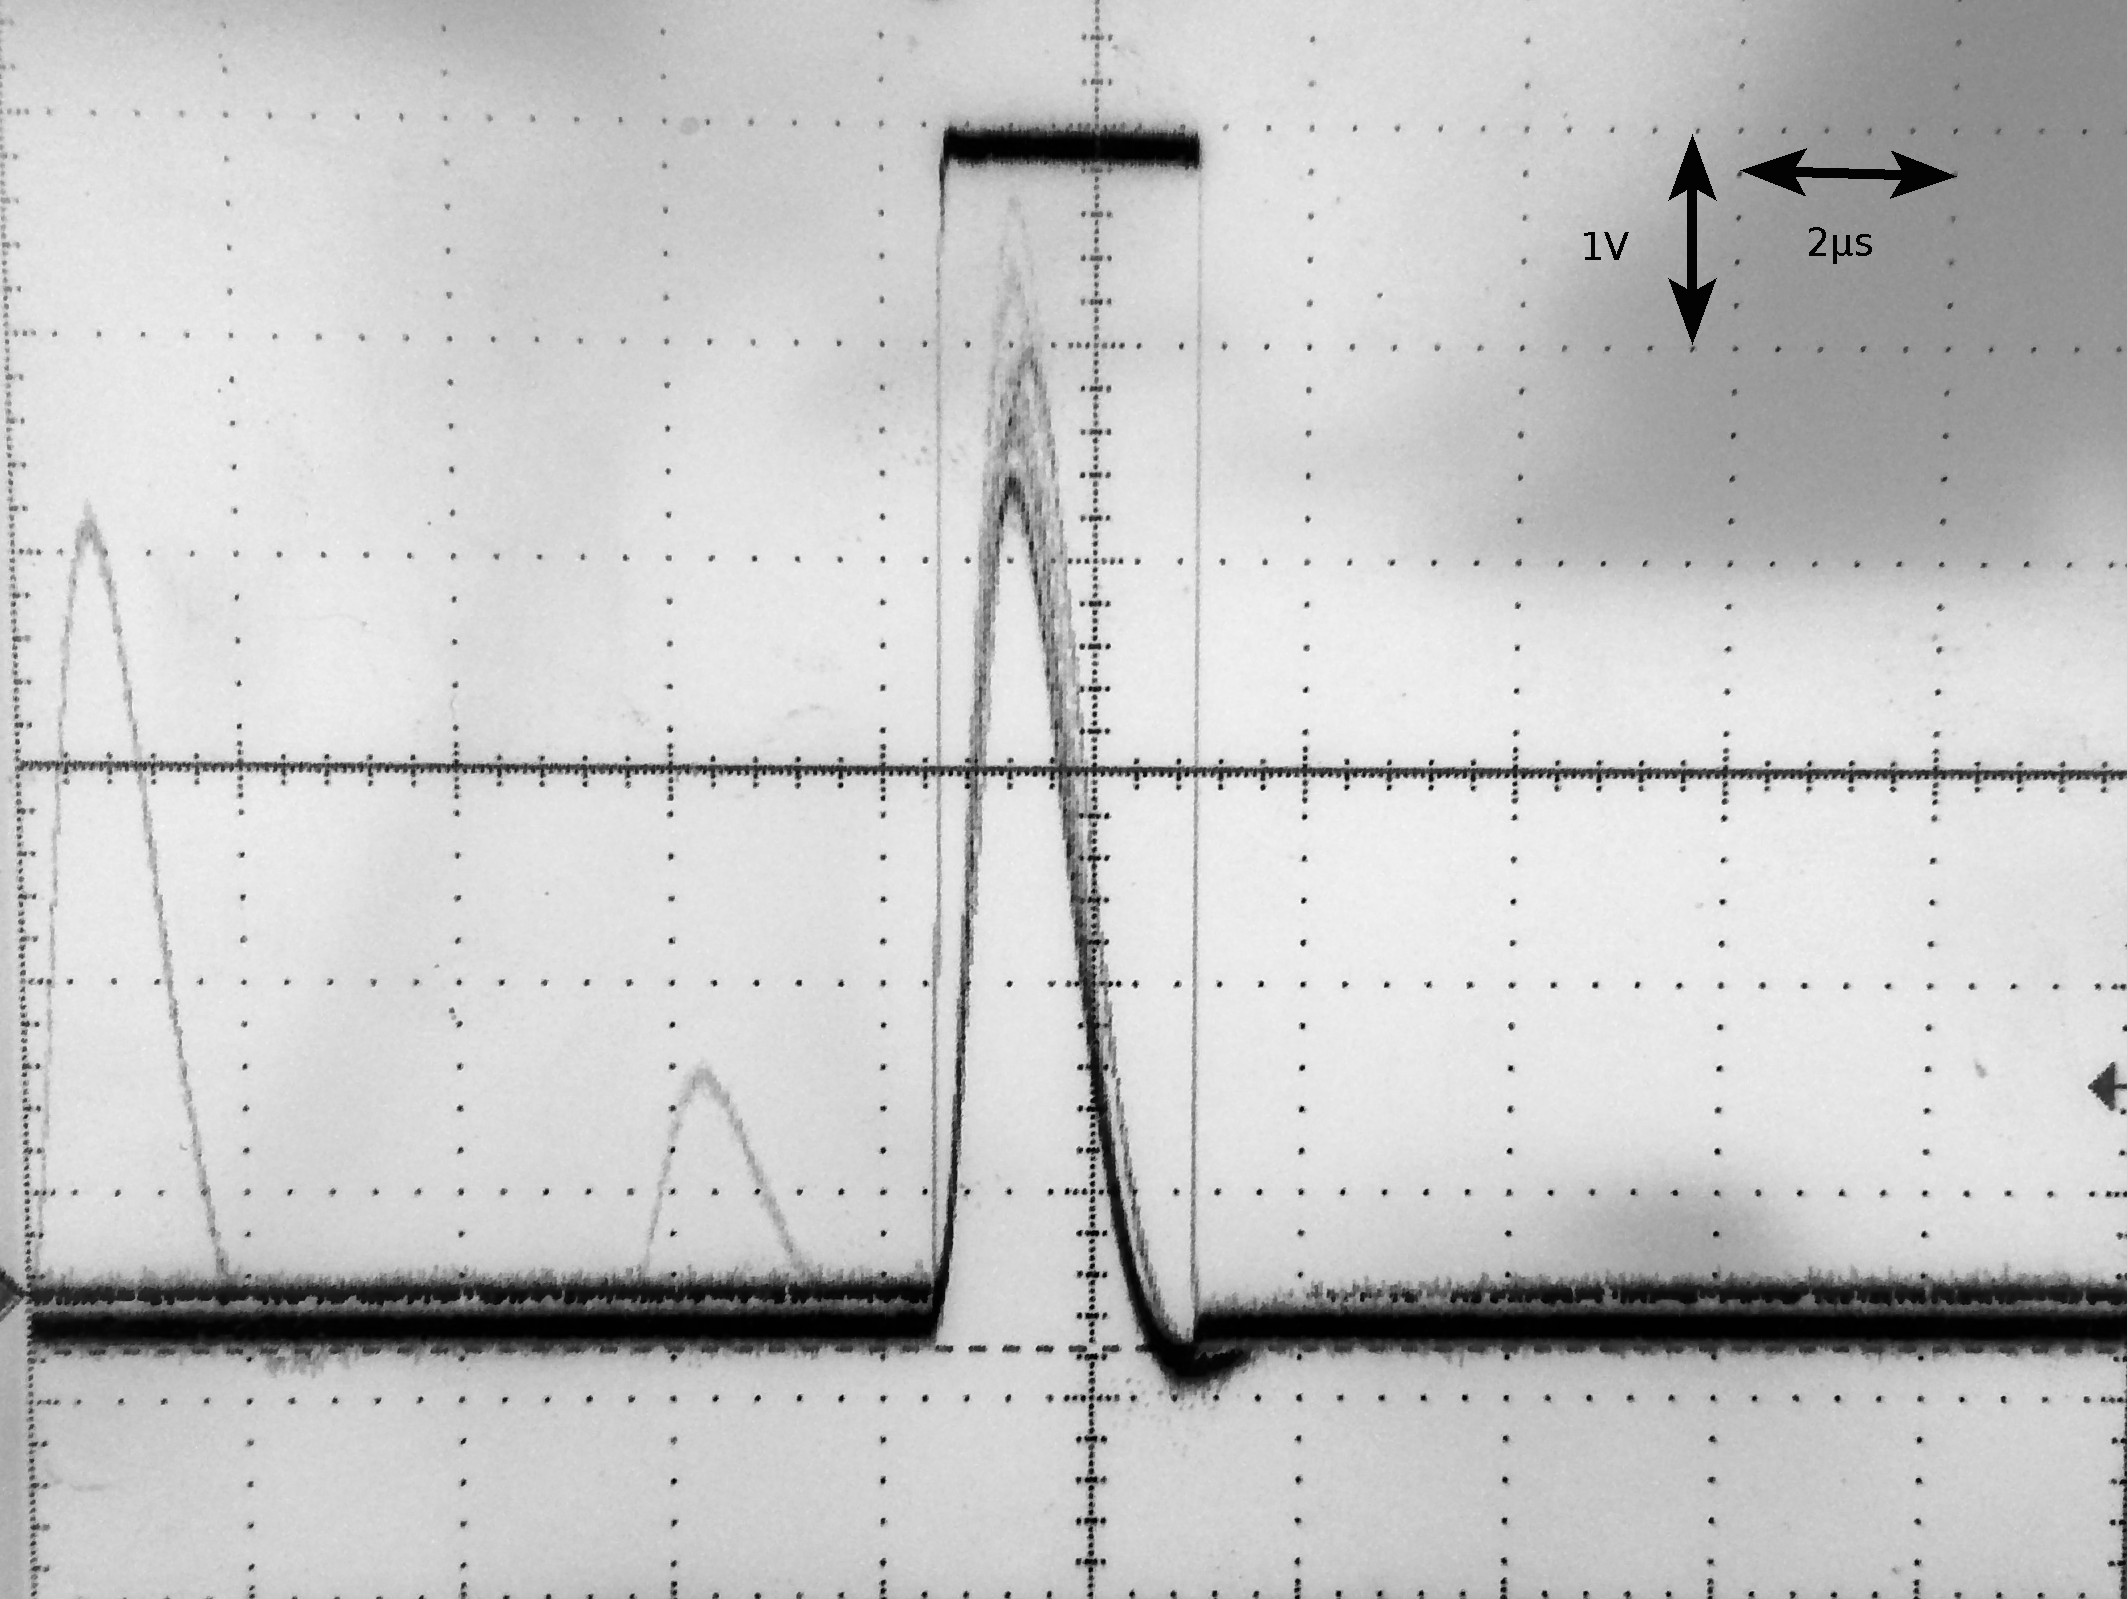
\includegraphics[width=0.45\textwidth]{Figures/sca_analog_left.png}};
    \draw (-9,-1.25-1.6) rectangle (-7,-0.25-1.6);
    \draw (-8,-0.5-1.6) node {Slow-};
    \draw (-8,-1-1.6) node {Output};
    \draw (-7,-0.75-1.6)--(-6.5,-0.75-1.6)--(-6.5,-1-1.6)--(-6,-0.75-1.6)--(-6.5,-0.5-1.6)--(-6.5,-0.75-1.6);
    \draw (-6,-2.35)--(-5.5,-2.35)--(-5.5,-1.6)--(-5,-1.6);
    \draw (-5,-1.35) rectangle (-4,-1.85);
    \draw (-4.5,-1.6) node {Delay};
    \draw (-4,-1.6)--(-0.75,-1.6)--(-0.75,-1.85)--(-0.5,-1.85);
    \draw (-6,-2.35)--(-5,-2.35);
    \draw (-5,-2.1) rectangle (-4,-2.6);
    \draw (-4.5,-2.35) node {SCA};
    \draw (-4,-2.35)--(-3.5,-2.35);
    \draw (-3.5,-2.1) rectangle (-2.5,-2.6);
    \draw (-3,-2.35) node {GDG};
    \draw (-2.5,-2.35)--(-0.75,-2.35)--(-0.75,-1.99)--(-0.5,-1.99);
  \end{tikzpicture}
  \caption{Setup for the measurement of energy spectra.}
  \label{fig:sca_analog}
\end{figure}

Using this setup and the MCA we measure the spectra of the LYSO scintillator itself and that of $^{22}$Na. The same steps are repeated for the second detector. Then we adjust a delay such that the gate signals coming from both detectors are simultaneuos (figure \ref{fig:slow_coincidence}). After the measurements the windows of the SCA's are adjusted to filter out the \SI{511}{\kilo\electronvolt} line from the electron-positron annihilation.

\begin{figure}[h]
  \centering
  \begin{tikzpicture}
    \node at (3.25,0) {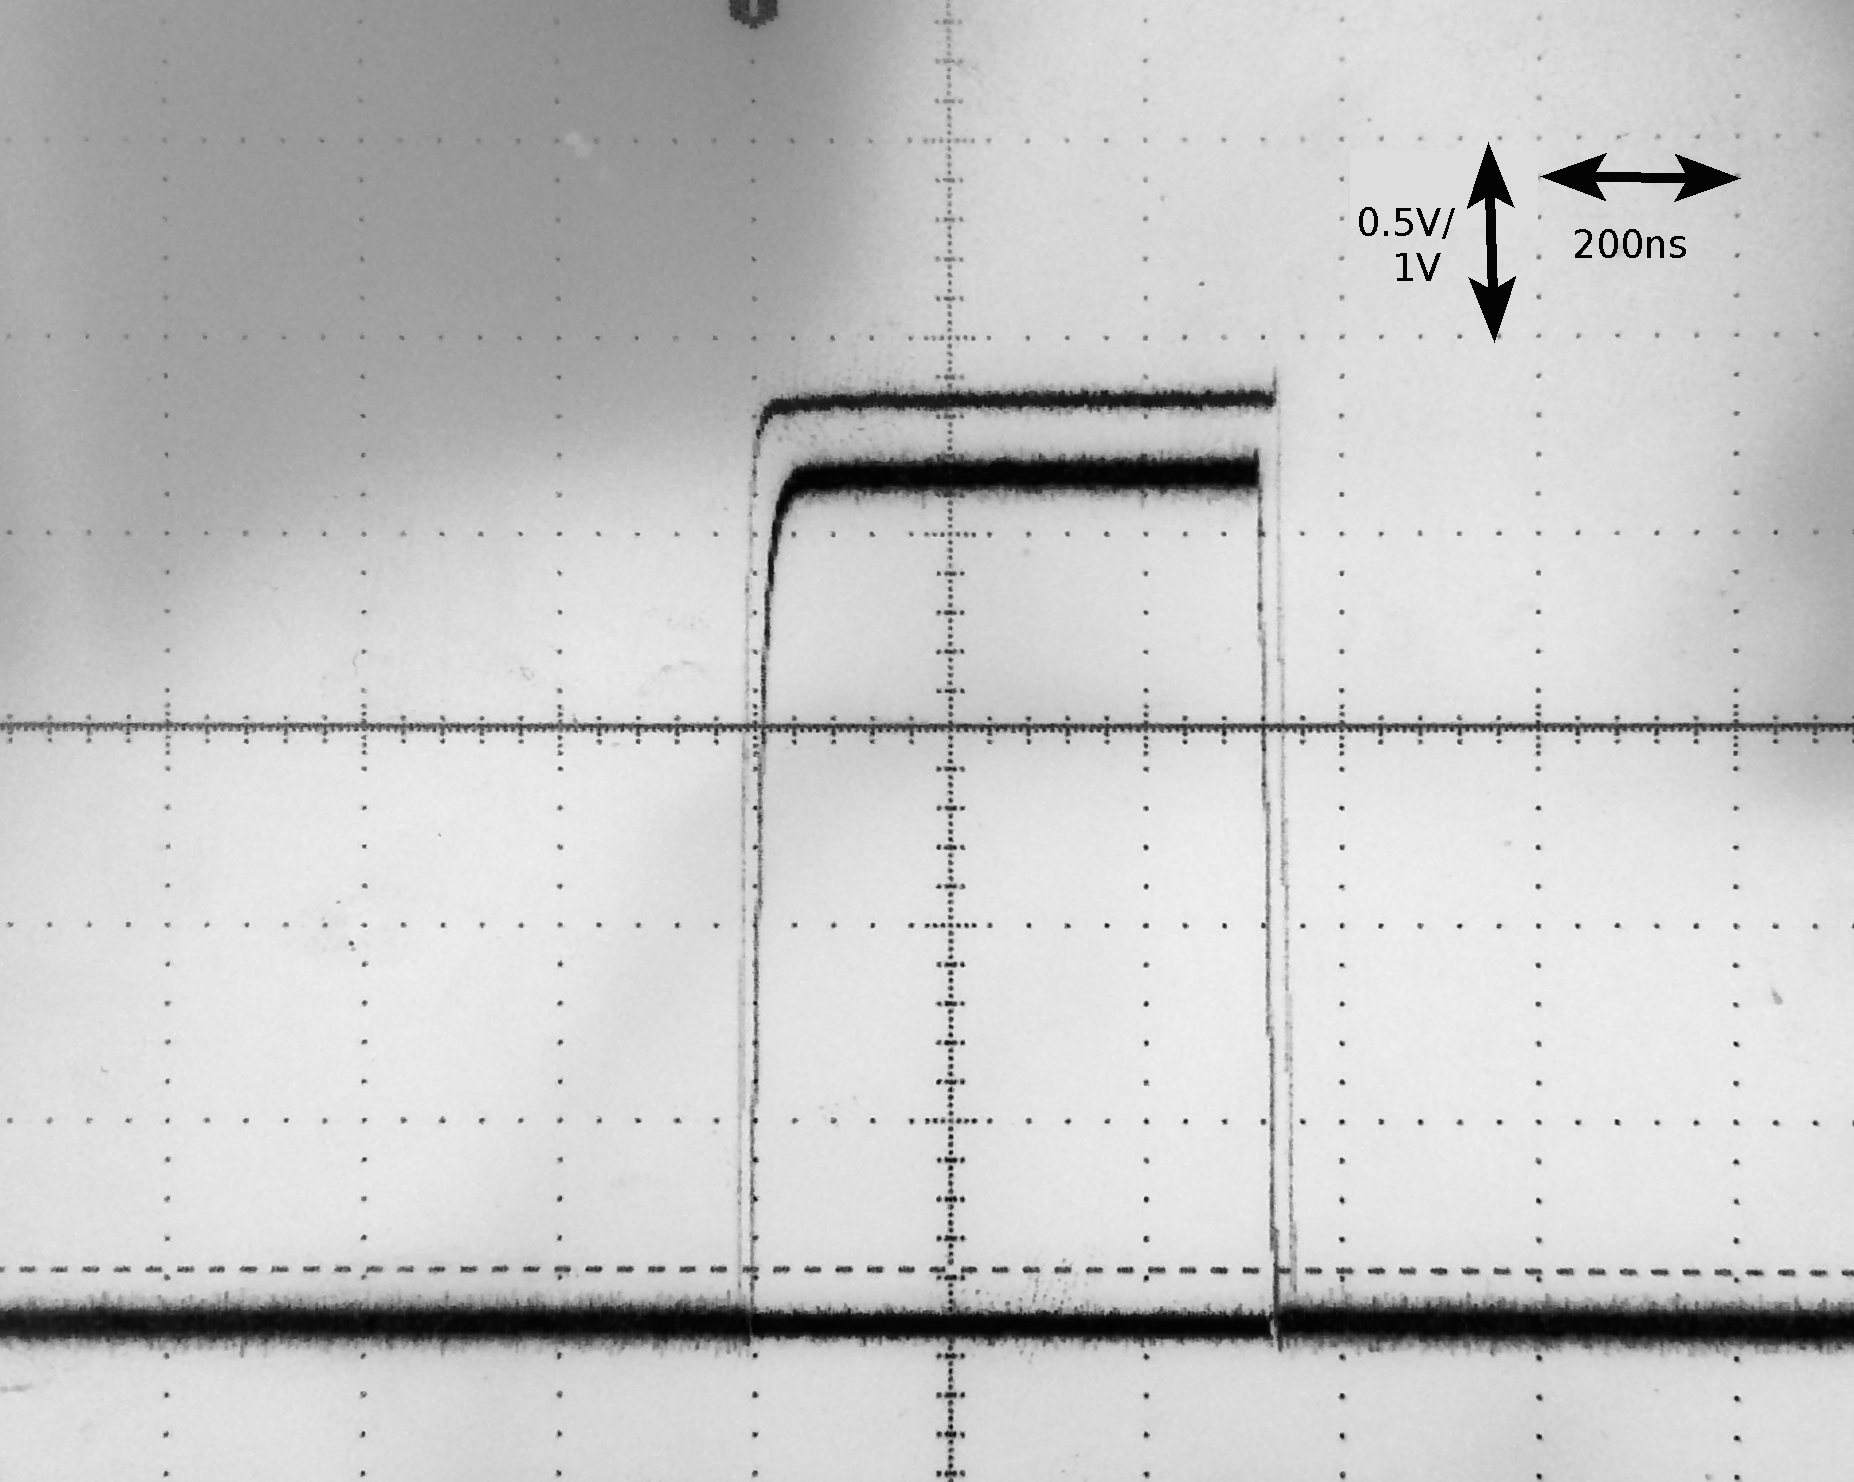
\includegraphics[width=0.45\textwidth]{Figures/slow_coincidence.png}};
    \draw (-9,-1.25-1.6) rectangle (-7,-0.25-1.6);
    \draw (-8,-0.5-1.6) node {L: Slow-};
    \draw (-8,-1-1.6) node {Ausgang};
    \draw (-7,-0.75-1.6)--(-6.5,-0.75-1.6)--(-6.5,-1-1.6)--(-6,-0.75-1.6)--(-6.5,-0.5-1.6)--(-6.5,-0.75-1.6);
    \draw (-6,-2.35)--(-5.5,-2.35);
    \draw (-6,-2.35)--(-5,-2.35);
    \draw (-5,-2.1) rectangle (-4,-2.6);
    \draw (-4.5,-2.35) node {SCA};
    \draw (-4,-2.35+3.15)--(-2.5,-2.35+3.15);
    \draw (-2.5,-2.35+3.15)--(-1.9,-2.35+3.15);
    \draw (-1.9,-2.35)--(-1.9,-2.35)--(-0.5,-2.35);

    \draw (-9,-1.25-1.6+3.15) rectangle (-7,-0.25-1.6+3.15);
    \draw (-8,-0.5-1.6+3.15) node {R: Slow-};
    \draw (-8,-1-1.6+3.15) node {Output};
    \draw (-7,-0.75-1.6+3.15)--(-6.5,-0.75-1.6+3.15)--(-6.5,-1-1.6+3.15)--(-6,-0.75-1.6+3.15)--(-6.5,-0.5-1.6+3.15)--(-6.5,-0.75-1.6+3.15);
    \draw (-6,-2.35+3.15)--(-5.5,-2.35+3.15);
    \draw (-6,-2.35+3.15)--(-5,-2.35+3.15);
    \draw (-5,-2.1+3.15) rectangle (-4,-2.6+3.15);
    \draw (-4.5,-2.35+3.15) node {SCA};
    \draw (-4,-2.35)--(-3.5,-2.35);
    \draw (-3.5,-2.1) rectangle (-2.5,-2.6);
    \draw (-3,-2.35) node {Delay};
    \draw (-2.5,-2.35)--(-1.9,-2.35);
    \draw (-1.9,0.8)--(-1.9,-2.3)--(-0.5,-2.3);
  \end{tikzpicture}
  \caption{Comparison of both slow-signals. The upper signal corresponds to the \SI{0.5}{\volt} signal.}
  \label{fig:slow_coincidence}
\end{figure}

\subsection{Setup of Fast-Circuit}
The CFD threshold of one side must be adjusted such that one has a good acceptance but cuts away as much noise as possible. We do this by making the threshold as high as possible without cutting the \SI{511}{\kilo\electronvolt} line\footnote{This is the most persistent line in the spectrum.} (figure \ref{fig:cfd}). It turns out that the chosen threshold is the maximal threshold possible. The same is done for the other side of the fast-circuit. \newpage

\begin{figure}[h]
  \centering
  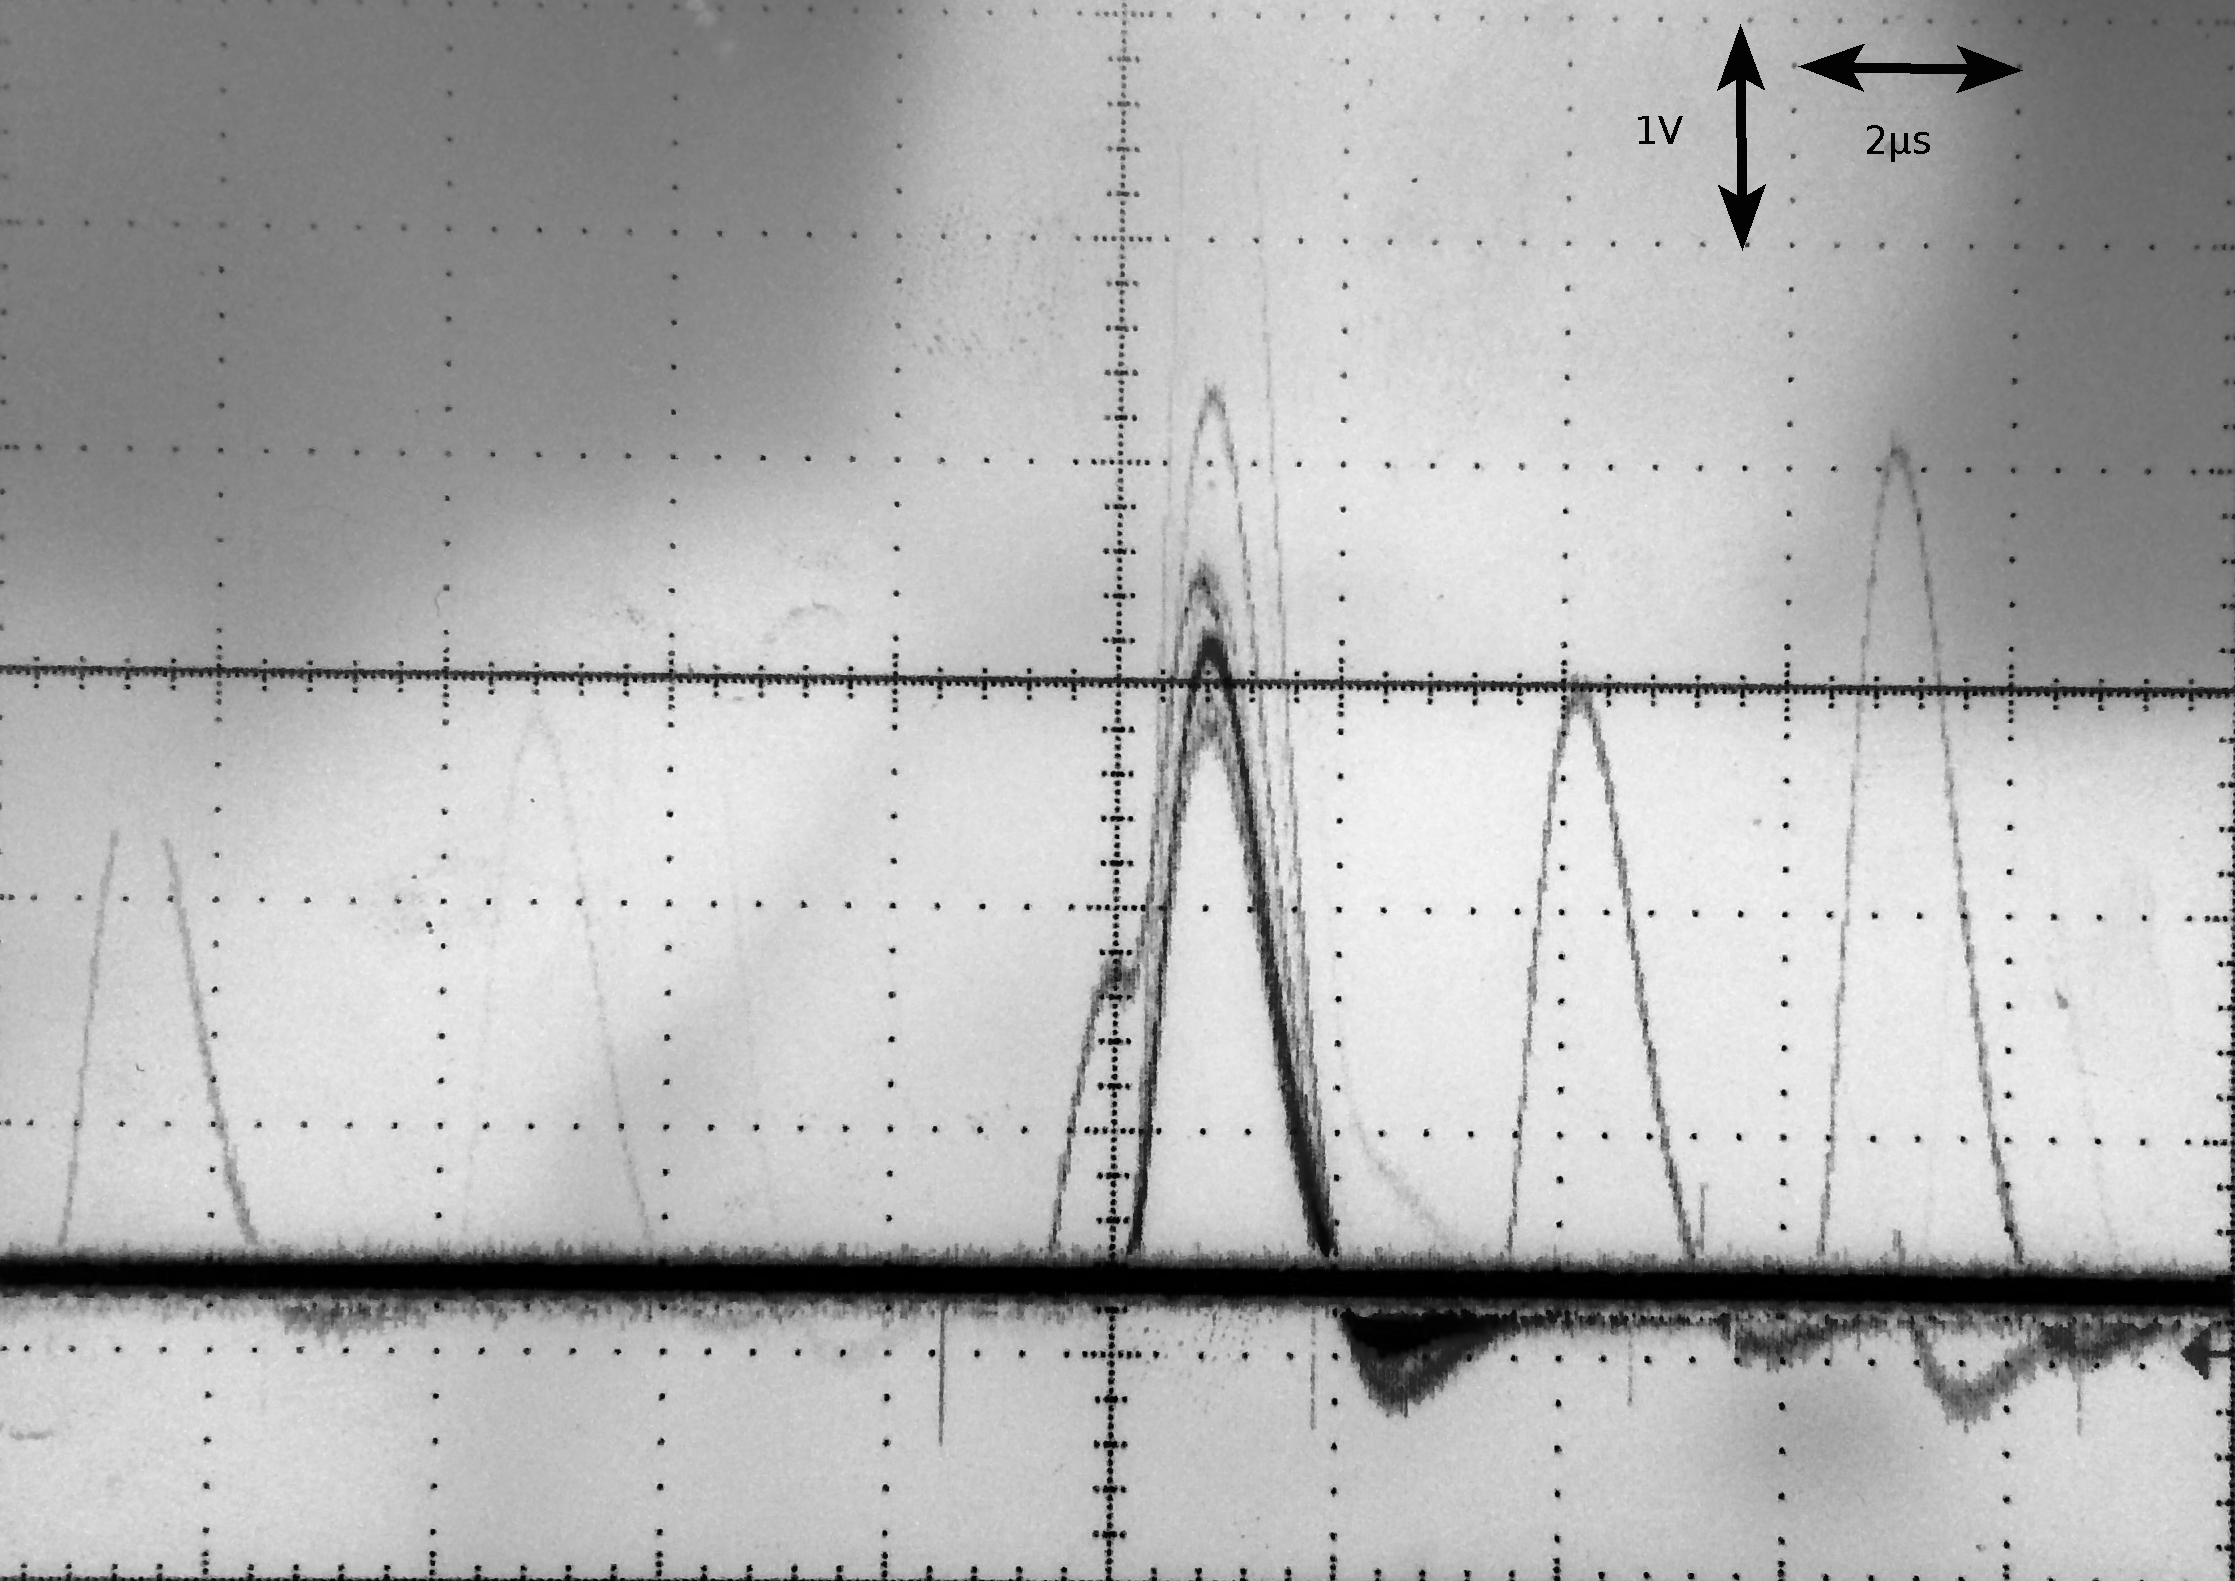
\includegraphics[width=0.5\textwidth]{Figures/cfd_left.png}
  \caption{CFD signal after setting the threshold.}
  \label{fig:cfd}
\end{figure}

To make sure that the start signal comes before the stop signal the time delay between both signals is set to approximate \SI{20}{\nano\second}. The signals can be seen in figure \ref{fig:delay_cfd}. 

\begin{figure}[h]
  \centering
  \begin{tikzpicture}
    \node at (3.25,1.3) {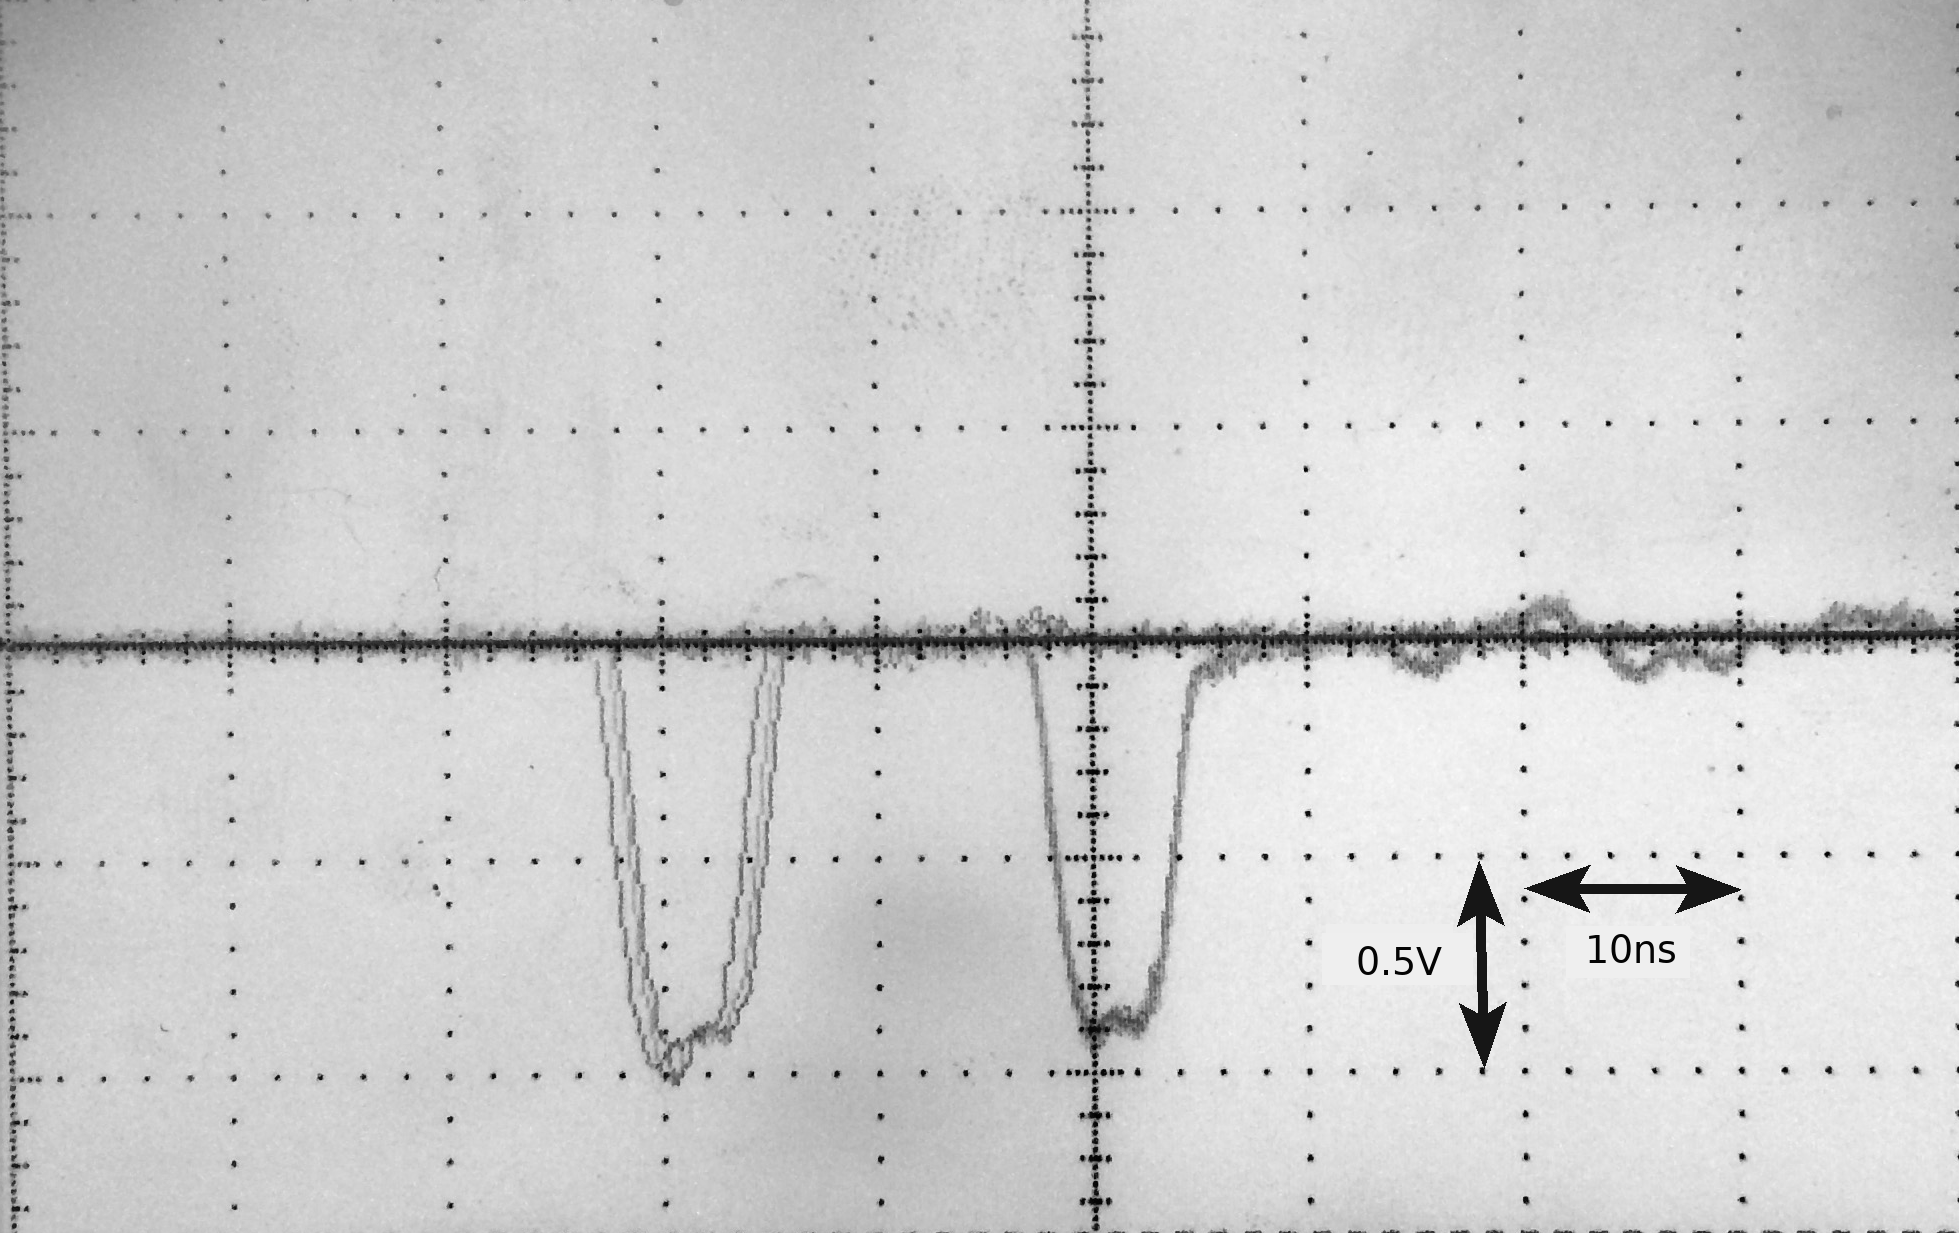
\includegraphics[width=0.45\textwidth]{Figures/cfd_delay.png}};
    \draw (-9,-1.25-1.6+3.95) rectangle (-7,-0.25-1.6+3.95);
    \draw (-8,-0.5-1.6+3.95) node {R: Fast-};
    \draw (-8,-1-1.6+3.95) node {Output};
    \draw (-7,-0.75-1.6+3.95)--(-6,-0.75-1.6+3.95);
    \draw (-6,-2.35+3.95)--(-5.5,-2.35+3.95);
    \draw (-6,-2.35+3.95)--(-5,-2.35+3.95);
    \draw (-5,-2.1+3.95) rectangle (-4,-2.6+3.95);
    \draw (-4.5,-2.35+3.95) node {CFD};
    \draw (-4,-2.35+3.95)--(-2.5,-2.35+3.95);
    \draw (-2.5,-2.35+3.95)--(-2,-2.35+3.95)--(-2,1.23)--(-0.5,1.23);
    
    \draw (-9,-1.25-1.6+2.8) rectangle (-7,-0.25-1.6+2.8);
    \draw (-8,-0.5-1.6+2.8) node {L: Fast-};
    \draw (-8,-1-1.6+2.8) node {Output};
    \draw (-7,-0.75-1.6+2.8)--(-6,-0.75-1.6+2.8);
    \draw (-6,-2.35+2.8)--(-5.5,-2.35+2.8);
    \draw (-6,-2.35+2.8)--(-5,-2.35+2.8);
    \draw (-5,-2.1+2.8) rectangle (-4,-2.6+2.8);
    \draw (-4.5,-2.35+2.8) node {CFD};
    \draw (-4,-2.35+2.8)--(-3.5,-2.35+2.8);
    \draw (-3.5,-2.1+2.8) rectangle (-2.5,-2.6+2.8);
    \draw (-3,-2.35+2.8) node {Delay};
    \draw (-2.5,-2.35+2.8)--(-2,-2.35+2.8)--(-2,1.17)--(-0.5,1.17);
  \end{tikzpicture}
  \caption{Delay between start- and stop-signal.}
  \label{fig:delay_cfd}
\end{figure}

We connect the start- and stop-signal to the TAC\footnote{It is important to use the same cables as before such that the delay remains to be about \SI{20}{\nano\second}.} and set the time range of the TAC to \SI{50}{\nano\second}. We then adjust the simultaneousness of the TAC-signal and the coincidence of the slow-circuit with the GDG. The result can be seen in figure \ref{fig:slow_fast}. The setup is now ready for the time calibration. \newpage

\begin{figure}[h]
  \centering
  \begin{tikzpicture}
    \node at (3.25,1.1) {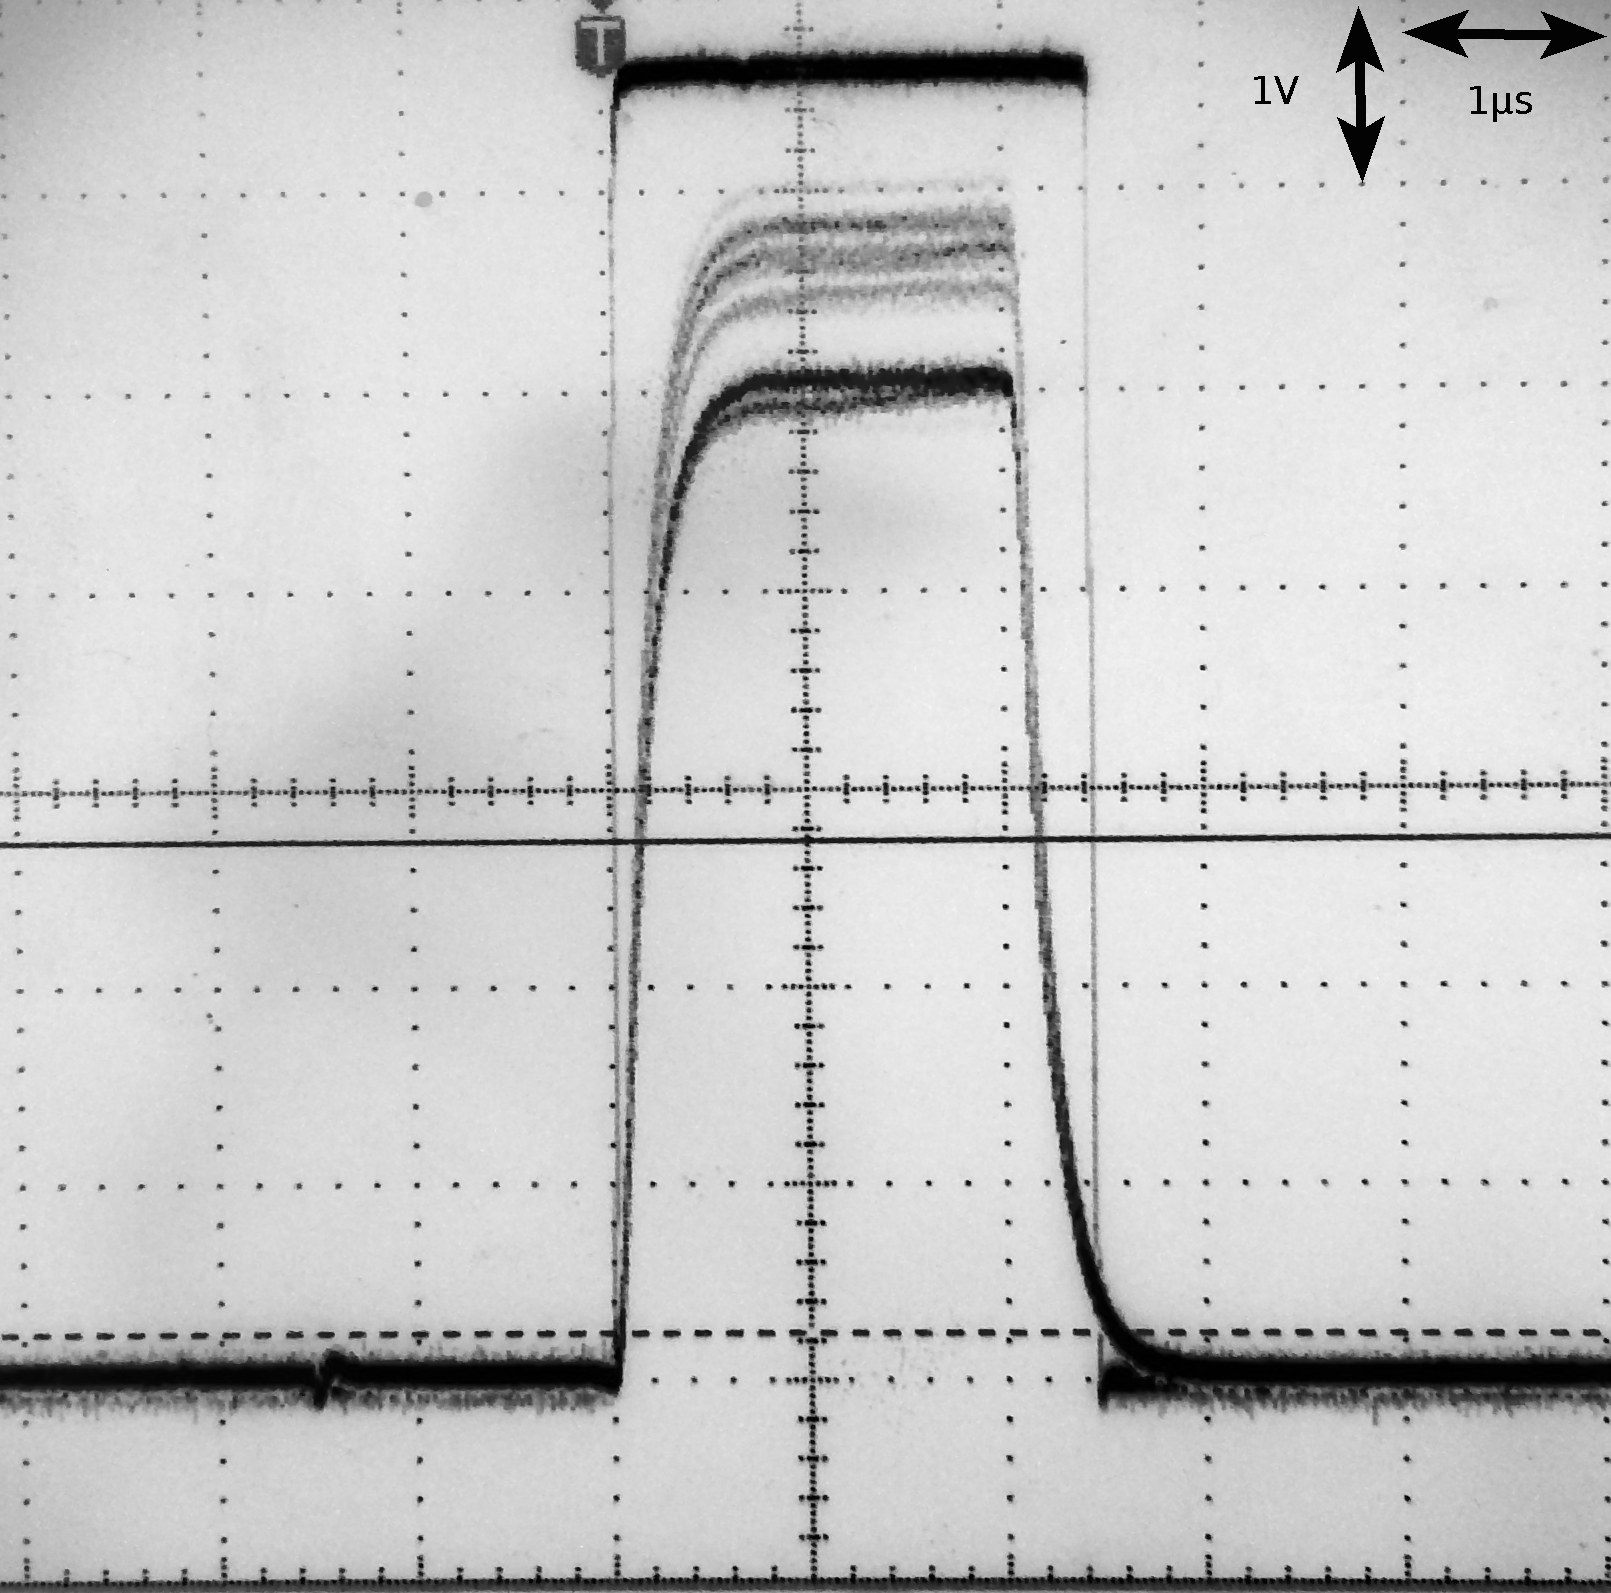
\includegraphics[width=0.45\textwidth]{Figures/coinc_tac.png}};
    \draw (-9,-1.25-1.6+3.95) rectangle (-7,-0.25-1.6+3.95);
    \draw (-8,-0.5-1.6+3.95) node {R: Fast-};
    \draw (-8,-1-1.6+3.95) node {Ausgang};
    \draw (-7,-0.75-1.6+3.95)--(-1-5,-0.75-1.6+3.95);
    \draw (-1-5,-2.1+3.95) rectangle (-1-4,-2.6+3.95);
    \draw (-1-4.5,-2.35+3.95) node {CFD};
    \draw (-1-4,-2.35+3.95)--(-1-1.4+0.5,-2.35+3.95)--(-1.9,0);
    \draw (-9,-1.25-1.6+2.8) rectangle (-7,-0.25-1.6+2.8);
    \draw (-8,-0.5-1.6+2.8) node {L: Fast-};
    \draw (-8,-1-1.6+2.8) node {Ausgang};
    \draw (-7,-0.75-1.6+2.8)--(-1-5,-0.75-1.6+2.8);
    \draw (-1-5,-2.1+2.8) rectangle (-1-4,-2.6+2.8);
    \draw (-1-4.5,-2.35+2.8) node {CFD};
    \draw (-1-4,-2.35+2.8)--(-1-3.5,-2.35+2.8);
    \draw (-1-3.5,-2.1+2.8) rectangle (-1-2.5,-2.6+2.8);
    \draw (-1-3,-2.35+2.8) node {Delay};
    \draw (-1-2.5,-2.35+2.8)--(-1-1.4,-2.35+2.8)--(-2.4,0);
    \draw (-2.65,0) rectangle (-1.65,-0.5);
    \draw (-2.15,-0.25) node {TAC};
    \draw (-2.15,-0.5)--(-2.15,-1.2)--(-0.625,-1.2)--(-0.625,-1.56)--(-0.5,-1.56);

    \draw (-9,-1.25-1.6+3.95-2.525-0.45) rectangle (-7,-0.25-1.6+3.95-2.525-0.45);
    \draw (-8,-0.5-1.6+3.95-2.525-0.45) node {R: Slow-};
    \draw (-8,-1-1.6+3.95-2.525-0.45) node {Ausgang};
    \draw (-7,-0.75-1.6+3.95-2.525-0.45)--(-6.75,-0.925-0.45)--(-6.75,-1.175-0.45)--(-6.25,-0.925-0.45)--(-6.75,-0.675-0.45)--(-6.75,-0.925-0.45);
    \draw (-6.25,-0.925-0.45)--(-1-5,-0.75-1.6+3.95-2.525-0.45);
    \draw (-1-5,-2.1+3.95-2.525-0.45) rectangle (-1-4,-2.6+3.95-2.525-0.45);
    \draw (-1-4.5,-2.35+3.95-2.525-0.45) node {SCA};
    \draw (-1-4,-2.35+3.95-2.525-0.45)--(-3.25,-2.35+3.95-2.525-0.45)--(-3.25,-1.4-0.45)--(-3,-1.4-0.45);
    \draw (-9,-1.25-1.6+2.8-2.525-0.45) rectangle (-7,-0.25-1.6+2.8-2.525-0.45);
    \draw (-8,-0.5-1.6+2.8-2.525-0.45) node {L: Slow-};
    \draw (-8,-1-1.6+2.8-2.525-0.45) node {Ausgang};
    \draw (-7,-0.75-1.6+2.8-2.525-0.45)--(-6.75,-0.925-1.15-0.45)--(-6.75,-1.175-1.15-0.45)--(-6.25,-0.925-1.15-0.45)--(-6.75,-0.675-1.15-0.45)--(-6.75,-0.925-1.15-0.45);
    \draw (-6.25,-0.925-1.15-0.45)--(-1-5,-0.75-1.6+2.8-2.525-0.45);
    \draw (-1-5,-2.1+2.8-2.525-0.45) rectangle (-1-4,-2.6+2.8-2.525-0.45);
    \draw (-1-4.5,-2.35+2.8-2.525-0.45) node {SCA};
    \draw (-1-4,-2.35+2.8-2.525-0.45)--(-1-3.5,-2.35+2.8-2.525-0.45);
    \draw (-1-3.5,-2.1+2.8-2.525-0.45) rectangle (-1-2.5,-2.6+2.8-2.525-0.45);
    \draw (-1-3,-2.35+2.8-2.525-0.45) node {Delay};
    \draw (-1-2.5,-2.35+2.8-2.525-0.45)--(-3.25,-2.35+2.8-2.525-0.45)--(-3.25,-1.6-0.45)--(-3,-1.6-0.45);
    \draw (-3,-1.75-0.45) rectangle (-2,-1.25-0.45);
    \draw (-2.5,-1.5-0.45) node {Coinc.};
    \draw (-2,-1.5-0.45)--(-1.75,-1.5-0.45);
    \draw (-1.75,-1.75-0.45) rectangle (-0.75,-1.25-0.45);
    \draw (-1.25,-1.5-0.45) node {GDG};
    \draw (-0.75,-1.95)--(-0.625,-1.95)--(-0.625,-1.59)--(-0.5,-1.59);
  \end{tikzpicture}
  \caption{Coincidence-signal of the slow-circuit and TAC-signal of the fast-circuit.}
  \label{fig:slow_fast}
\end{figure}

\subsection{Time Calibration}
For the time calibration we record a prompt curve with the MCA. This is done ba varying the delay of the slow-circuit in steps of \SI{4}{\nano\second} while measuring the TAC-signal. The resulting spectrum consists of multiple peaks each seperated by \SI{4}{\nano\second} to the neighbouring peaks.

\subsection{Measurement of Time Constant}
For the temperature dependence of the lifetime spectrum we need to heat the indium sample to different temperatures. To do so we first measure the time constant of the system by setting the minimal heating power and measuring the temperature every \SI{30}{\second}.

\subsection{Lifetime Measurement}
For our final measurement we adjust one SCA (the left one) to filter out the \SI{1275}{\kilo\electronvolt} line from the $2^+ \rightarrow 0^+$ transition in $^{22}$Ne. This signal is the start-signal for our TAC. The right detector is already set to measure the \SI{511}{\kilo\electronvolt} line from the electron-positron annihilation. With this setup we measure the lifetime spectrum for different temperatures.
